%===================================== CHAP 5 =================================


\chapter{Solution Framework} \label{chapter_solution_approach}

The FPLDP is a complex problem with a high degree of uncertainty. In each gameweek a large range of decisions must be optimized. Compared to other Fantasy Sports, the gamechips make it even more complicated. The objective of the model presented in Chapter 4 is to maximize the number of expected points. If the model is run ex-post, the model yields the optimal solution as the realized points are known. However, in order to compete in FPL, decisions must be made ex-ante. Thus, estimations of expected points and strategies for when the gamechips should be played are required. The aim of this chapter is to provide such input and propose a solution method in order to maximize performance over the entire season. 

\newpar
In the first section of this chapter, we present an overview of the solution approach suggested. In Section \ref{Player_Performance}, three different methods for forecasting player performance are described. Finally, in the Sections \ref{Ch.5_Game_chips} and \ref{Ch.5_Variance_tradeoff}, respectively, methods for implementing gamechips and handling risk are proposed.


\section{Solution Approach}

As stochastic programming models seek to leverage probability distribution of uncertain parameters, they are regarded as more computational demanding than deterministic programming models \citep{Shapiro}. A common method for solving a stochastic model is by use of scenario generation. For the FPLDP, the number of scenarios explodes even for a modest number of scenarios. With only two scenarios in a gameweek, the number of scenarios already reaches over 1 million for 20 gameweeks ($2^{20} = 1\,048\,576$). Therefore, solving a stochastic model over a whole season is infeasible. Hence, we have decided to solve the FPLDP with a deterministic approach. It is solved in a rolling horizon framework where decisions are implemented for one gameweek at a time. When decisions are optimized for a given gameweek, a certain number of gameweeks ahead is considered and forecasts of realized points are generated. Furthermore, strategies for when to use gamechips and a method for incorporating risk are added to the mathematical model.
\newpar


When using a forecast to estimate the expected value of a player's points, the objective function described in Section \ref{mathematical_model} is simplified from: 

\begin{equation*}
\smaller
\begin{aligned}
\text{max} \; z ={} & \EX_{\omega} \Big\lbrack\sum\limits_{p \in \mathcal{P}} \sum\limits_{t \in \mathcal{T}} \Big( \mathlarger{\rho}_{pt}(\omega)y_{pt} + \mathlarger{\rho}_{pt}(\omega)f_{pt} + \epsilon  \mathlarger{\rho}_{pt}(\omega)h_{pt} + \sum_{l \in \mathcal{L}}\kappa_{l} \mathlarger{\rho}_{pt}(\omega)g_{ptl} \\ 
&  + 2 \mathlarger{\rho}_{pt}(\omega)c_{pt} \Big)  \Big\rbrack \\ 
& - R\sum_{t \in \mathcal{T}}\alpha_{t}
\end{aligned}
\end{equation*}

to 

\begin{equation*}
\smaller
\begin{aligned}
\text{max} \; z ={} &  \sum\limits_{p \in \mathcal{P}} \sum\limits_{t \in \mathcal{T}} \Big( \hat{\mathlarger{\rho}}_{pt} y_{pt} + \hat{\mathlarger{\rho}}_{pt} f_{pt} + \epsilon  \hat{\mathlarger{\rho}}_{pt} h_{pt} + \sum_{l \in \mathcal{L}}\kappa_{l} \hat{\mathlarger{\rho}}_{pt} g_{ptl} \\ 
& + 2 \hat{\mathlarger{\rho}}_{pt} c_{pt} \Big)  \\ 
& - R\sum_{t \in \mathcal{T}}\alpha_{t}
\end{aligned}
\end{equation*}


where $\hat{\rho}_{pt}$ denotes an estimation of expected points of each player $p$ in a gameweek $t$.

\newpar

\begin{comment}
The solution approach is divided into three different elements, as depicted in Figure \ref{fig:solution_approach}. The elements are:
\end{comment}

The solution approach is divided into three different elements. The elements are:

\begin{itemize}
    \item Forecast of player performance
    \item Gamechip strategies
    \item Risk handling
\end{itemize}

The forecasts are estimations of player performance, while the gamechip strategies are decisions regarding when to play the various gamechips. In order account for risk, additional constraints are introduced. By risk, we refer to the variance in overall team performance. The variance is induced by the variance in an individual player's predicted performance and from correlation in points obtained by players in the same or opposing teams.

\begin{comment}

\begin{figure}[H]
    \centering
    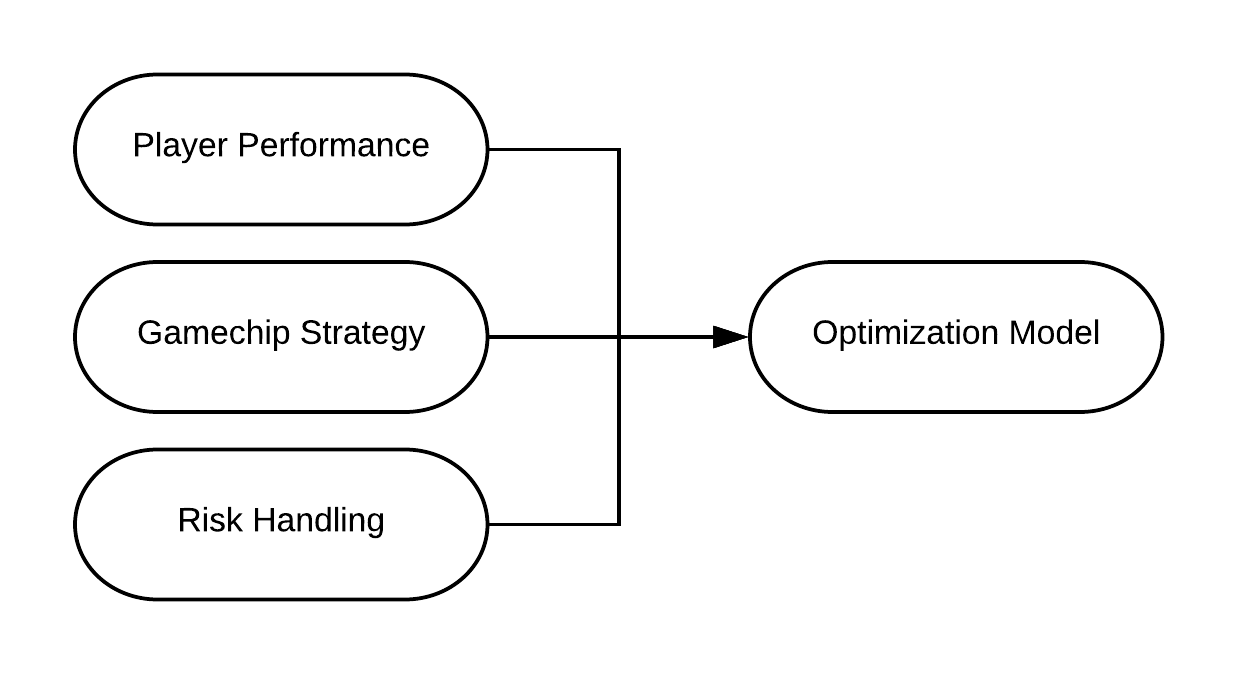
\includegraphics[scale = 0.65]{fig/chapter_5/solution_method.png}
    \caption{Elements in the solution approach.}
    \label{fig:solution_approach}
\end{figure}

\end{comment}
\newpar

In each gameweek, the mathematical model is solved for a set of gameweeks as new and updated information is incorporated. In this thesis, three forecast methods are considered to predict future player performances. The methods are: 
\begin{itemize}
    \item \textbf{Modified Average}. The solution approach suggested by \cite{Bonomo} is adapted and modified to FPL for prediction of a player's expected points.
    \item \textbf{Regression}. From a pool of explanatory variables related to the FPL, variables are selected and a linear regression model is fitted. 
    \item \textbf{Odds}. Bookmakers' odds can be adjusted to present a probability and consequently indicate future performance. Odds related to scorelines, goals, assists and yellow cards are utilized in order to estimate expected points. 
\end{itemize}

\newpar

Gamechip strategies are actions developed to decide when it is optimal to use the gamechips.  There exists limited literature on this topic. Consequently, there is a leeway for new ideas. Many interesting approaches could be adopted to decide the optimal use of gamechips. The approach adopted in this thesis is mainly qualitative and aim to take advantage of future gameweeks which are \textit{blank} or \textit{double}. The reader is reminded gameweek is blank when at least one team does not play, and a double if a team is featured more than once. 

\newpar

As described in Section \ref{Other_Relevant_Research}, there is a large resemblance between the FPLDP and the well known portfolio selection problem in financial theory. This is taken advantage of as risk is handled in an analogous manner.


\subsection{Rolling horizon}

The idea behind a rolling horizon heuristic is to split the problem into several sub-problems along a time axis, and then solve them in a chronological order taking into account the solution of the previous sub-problem. The heuristic suits problems with a long planning horizon where there are limited dependency between decisions made early and late in the planning horizon. Industrial planning and scheduling problems are common areas where the heuristic is used. The most important considerations are the number of sub-problems versus the length of each sub-problem, and which decisions to fix in each sub-problem. 

\begin{figure}[H]
    \centering
    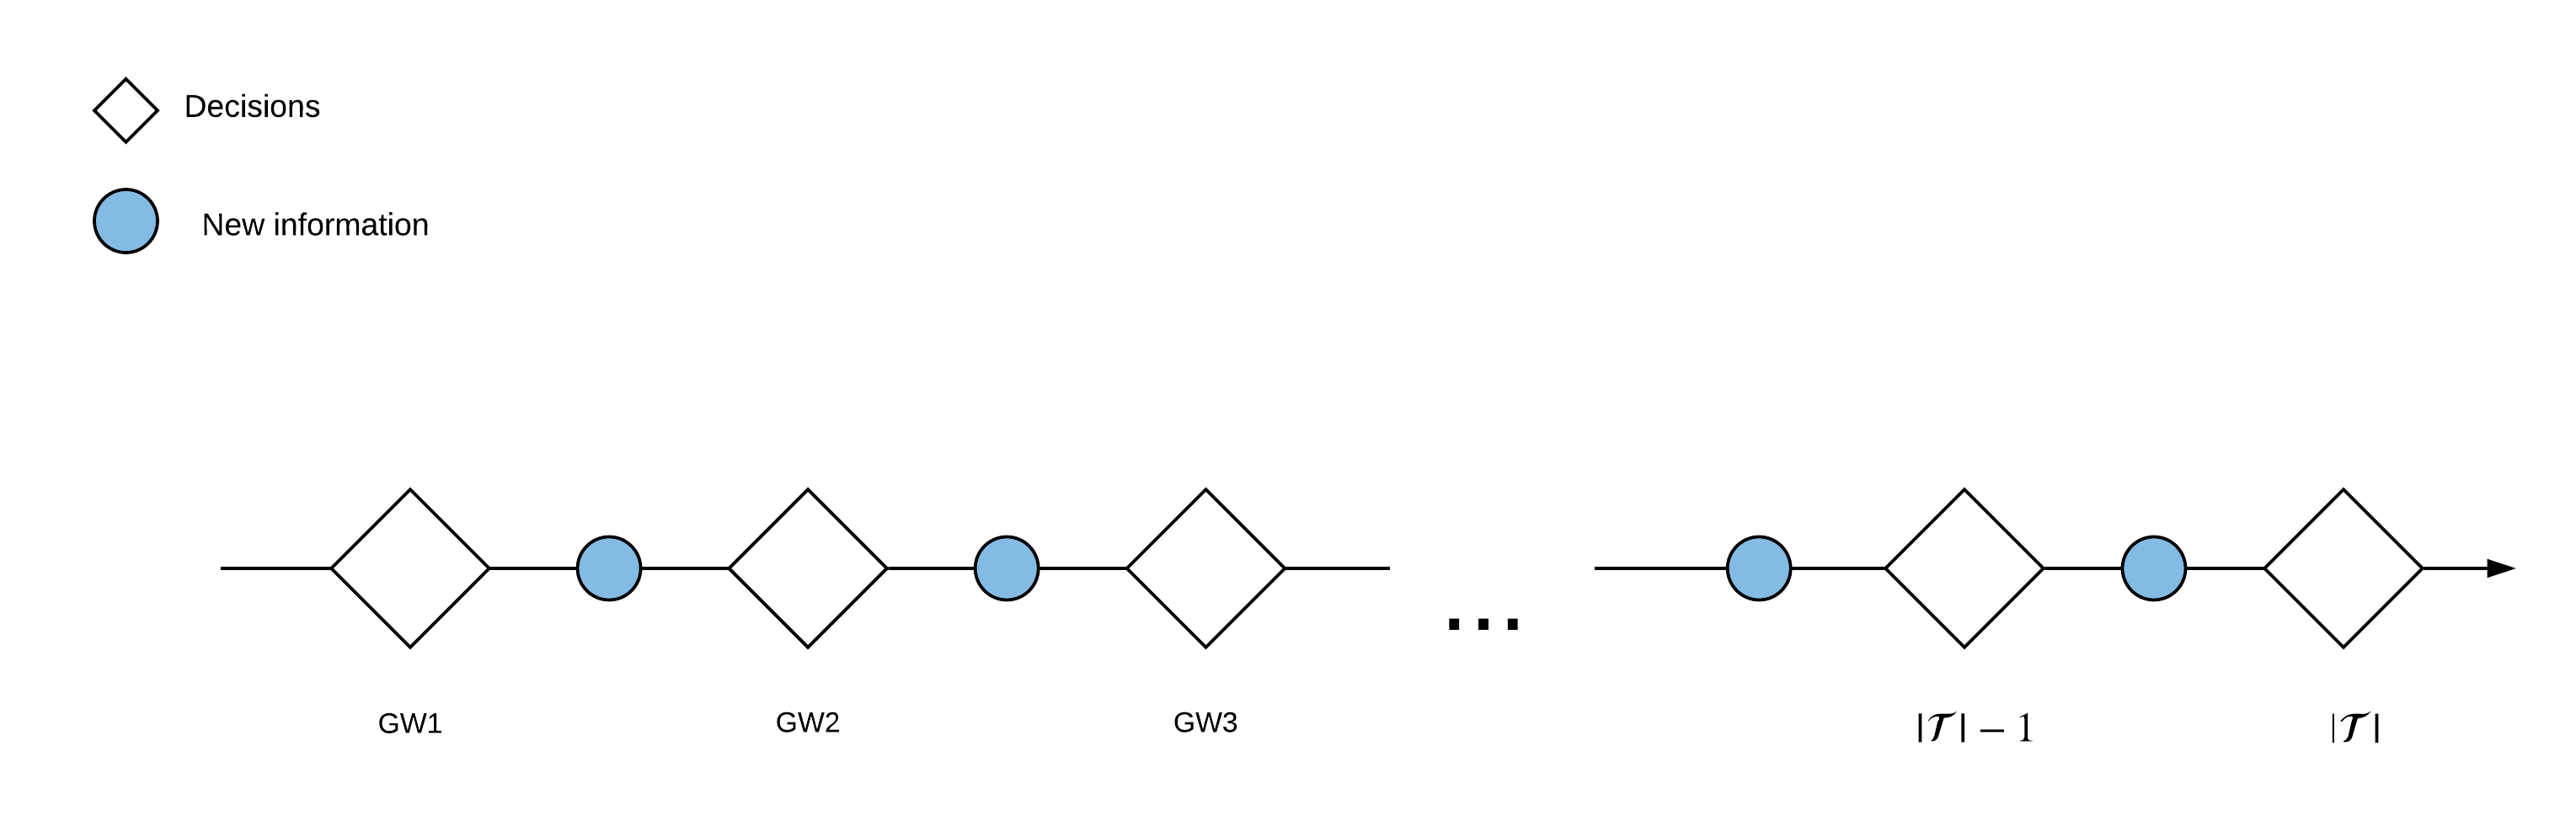
\includegraphics[scale = 0.47]{fig/chapter_5/Rolling_Horizon_Information_Flow.png}
    \caption{Information flow in the FPLDP.}
    \label{fig:information_flow}
\end{figure}

Rolling horizon is an appropriate solution method for FPLDP as managers are provided new information and face new decisions every gameweek. That is, each gameweek is a sub-problem. As shown in figure \ref{fig:information_flow}, decisions are made based on the information available. When a gameweek is played, updated information such as realized points, injuries and suspensions are made available. Hence, new decisions are made accordingly. Consequently, the problem is divided into $\mathcal{|T|}$ number of sub-problems along a time axis. That is, the decisions taken in a gameweek affect decisions in future gameweeks. However, decisions made early in the season have a limited impact on decisions made late in the season. It is fully possible to have a whole different selected squad in the last gameweeks compared to that of the first gameweeks. This is especially evident when the Wildcard is applied.

\newpar

In the rolling horizon heuristic, each sub-problem is solved over shorter sub-horizons for the whole season. This corresponds well to the FPLDP, as FPL managers often consider several gameweeks when making decisions. Each sub-horizon is split in two time periods ($TP$). The two \textit{TP}s are $TP_k^{C}$, which is the central period that will be implemented in sub-problem $k$, and the forecasting period $TP_k^{F}$. Before solving sub-problem $k+1$, variables $x$, $v$ and $q$ are frozen and used as input. The sub-horizon is shifted so that the first part of $TP_k^{F}$ becomes $TP_{k+1}^{C}$. If the central period and the forecasting period have equal length, the forecasting period becomes the new central period. 

\begin{enumerate}[label=(\roman*)]
    \item \textbf{Fixed period (FP)}. A gameweek where decisions have been implemented and used as input for the next sub-problem. These decisions are the players that are selected in a gameweek, $x$, the remaining budget variable, $v$, and the number of free transfers available, $q$.
    \item \textbf{Central period (CP)}. A gameweek where new decisions are implemented. The decisions include which players to include in the selected squad, $x$, determining the starting line-up, $y$, the choice of captain, $f$,  vice-captain, $h$, whether to use a gamechip or not and which substitution priority, $g$, to assign.  
    \item \textbf{Forecasting period (PP)}. To avoid making too myopic decisions, a predefined number of gameweeks are selected and input data such as expected points, variance and correlation are generated based on information available at that point in time. Decisions are made for these gameweeks, but not implemented.  The decisions are subject to change when new and updated information is available. 
\end{enumerate}

The FP, CP and PP in a sub-problem are illustrated graphically in figure \ref{fig:rolling_horizon}. In the figure, the predicted part overlaps the central part in order to illustrate that the input data in the central part is also predicted. The sub-horizon is set to 4 gameweeks in the figure. 

\begin{figure}[H]
    \centering
    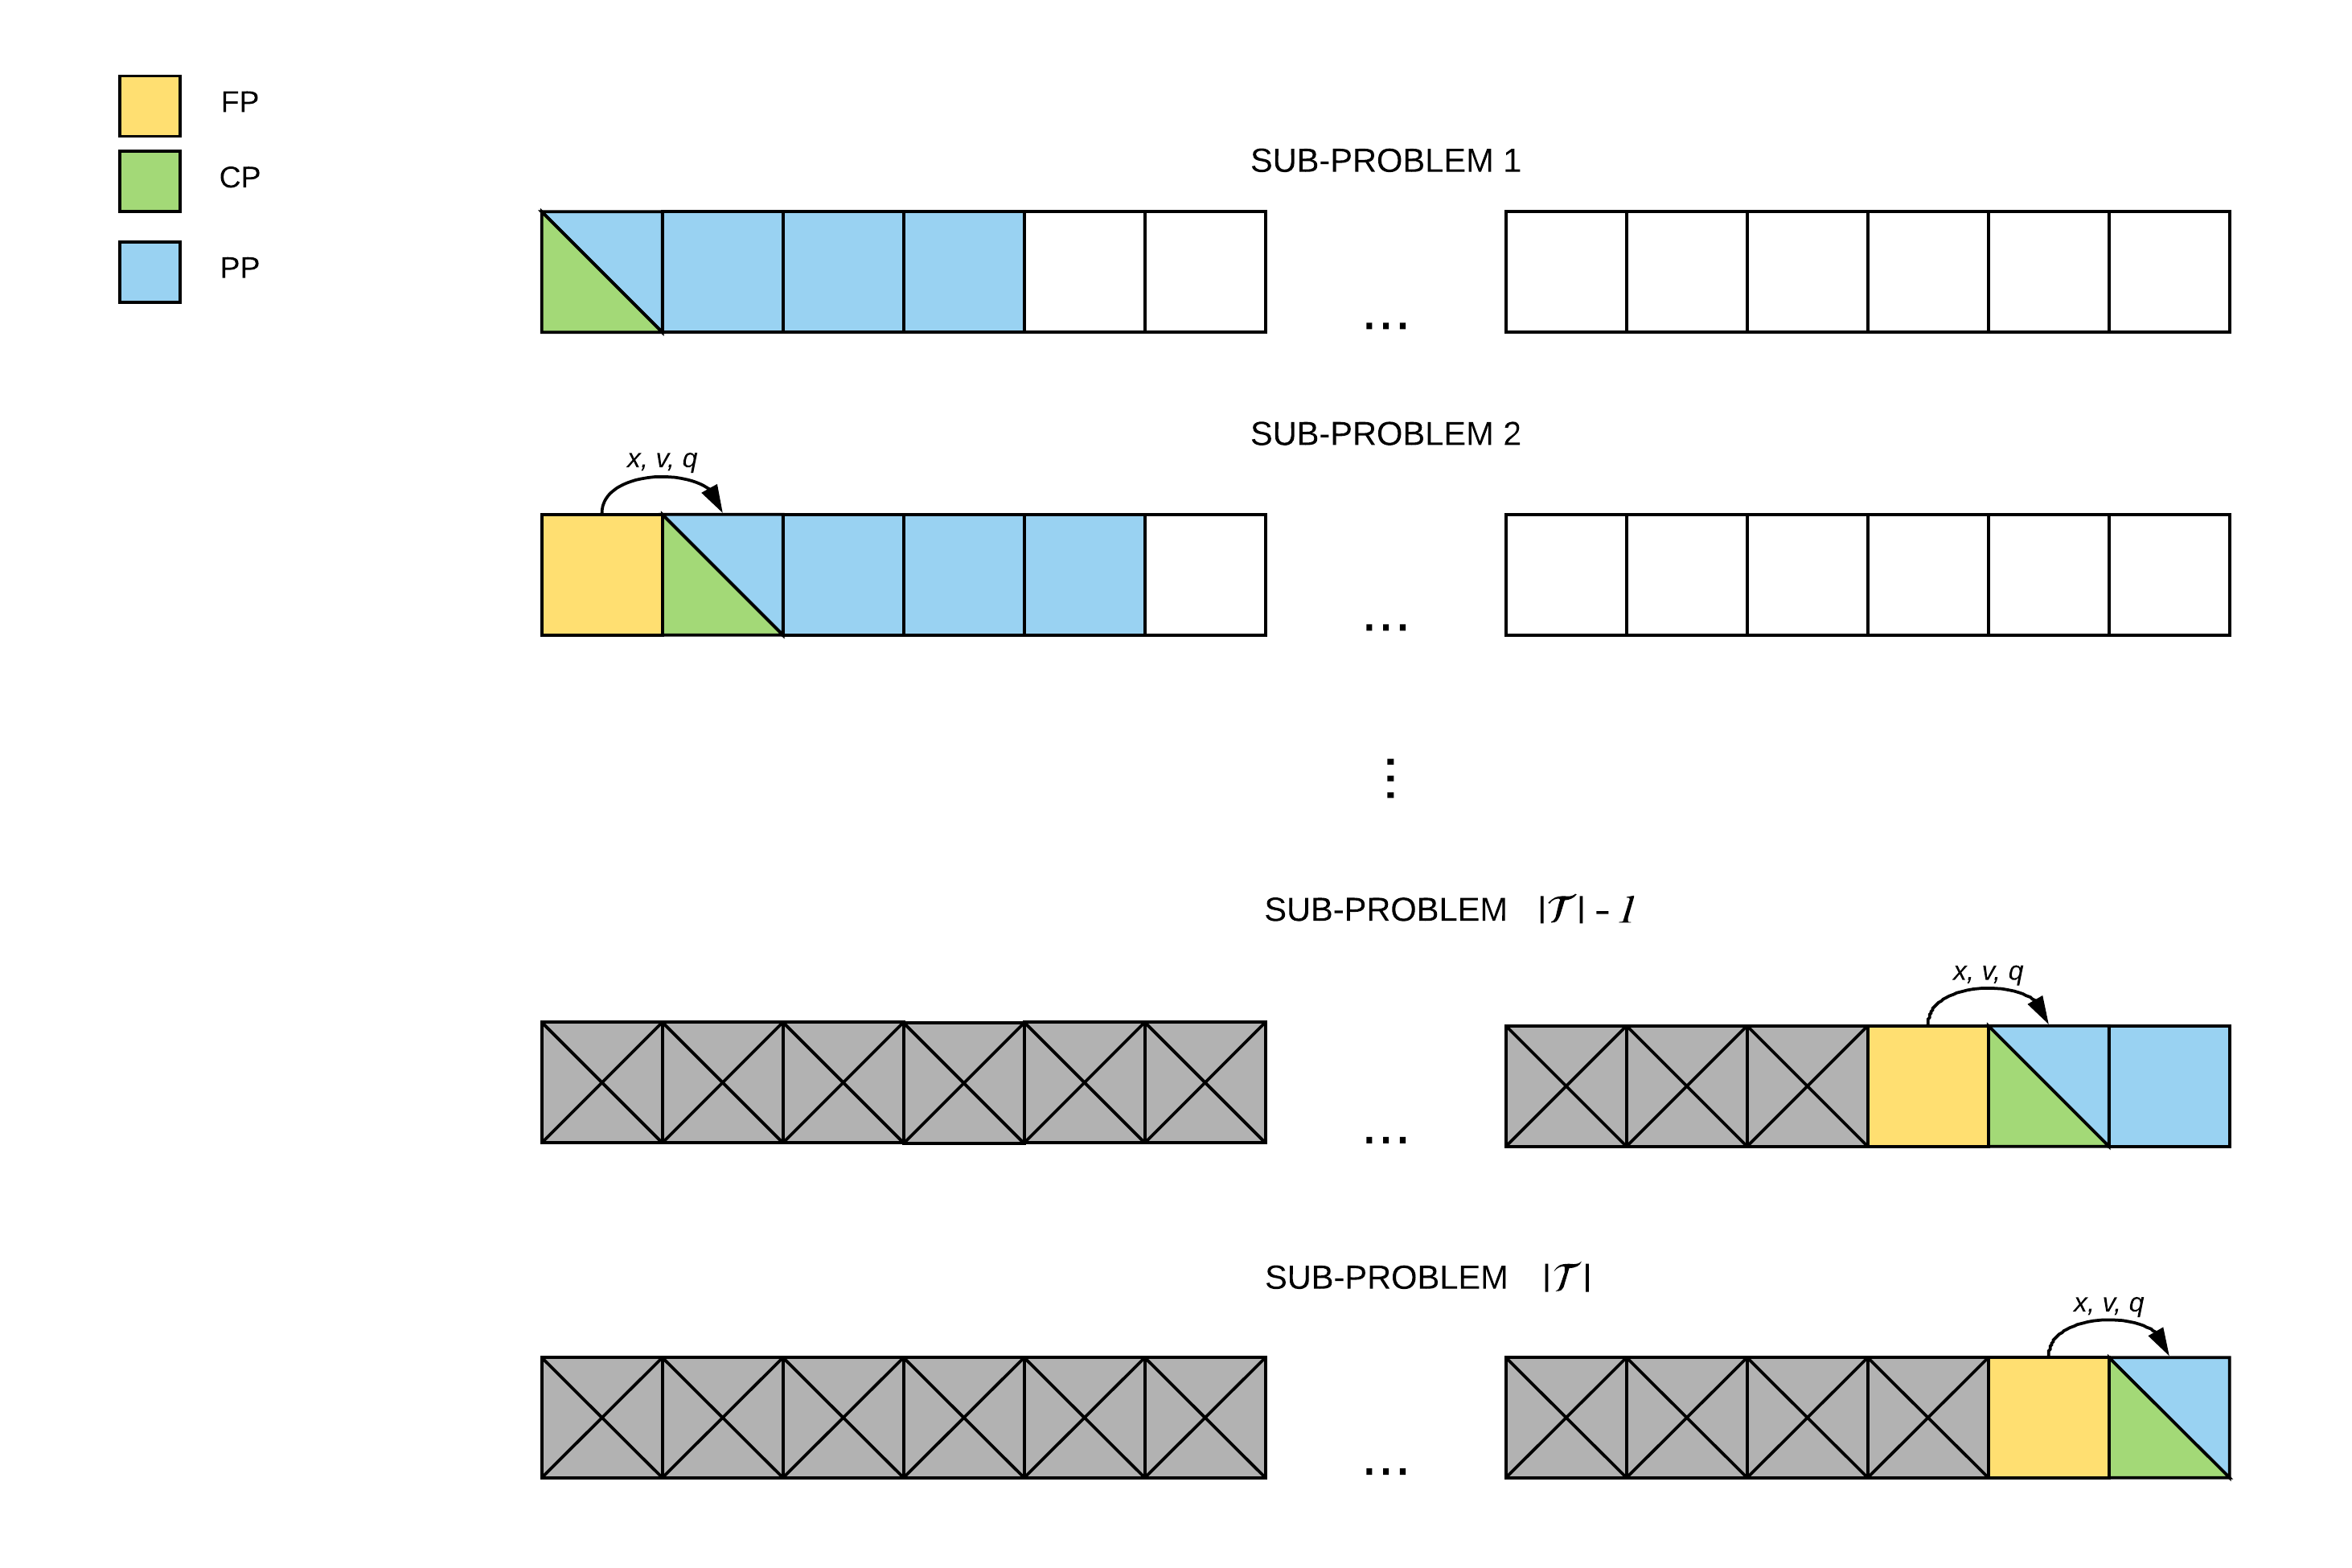
\includegraphics[scale = 0.47]{fig/chapter_5/rolling_horizon.png}
    \caption{Fixed-, central- and forecasting period in a sub-problem.}
    \label{fig:rolling_horizon}
\end{figure}

\newpar

An important decision is that of determining the length of the sub-horizon. Ideally, the sub-horizon should be for the remaining length of the season. However, due to the uncertainty of the forecasts, this is not necessarily ideal. Thus, several alternatives concerning the length of the sub-horizon should be tested in order to see what gives the best result. 

\newpar

By including forecasting, gamechip strategies and variance, we have arrived at a \textit{forecast-based optimization model} for the Fantasy Premier League Decision Problem. Algorithm \ref{alg:forecast_based_opt_model} gives a pseudo code for the forecast-based optimization model.


\newpar

\begin{algorithm}
\setstretch{1.35}
\caption{Forecast-based optimization model}
\begin{algorithmic}
\State{$k$ = 1} 
\While{$k$ $\leq$ $\mathcal{|T|}$}
    \State{Generate input data: expected points, variance and correlation for $TP_{k}^{C}$ and $TP_{k}^{F}$}
    \If{a gameweek in $TP_{k}^{F}$ is \textit{double} or \textit{blank}}
        \State{Implement gamechip strategy}
    \ElsIf{a gameweek in $TP_{k}^{F}$ according to Wildcard strategy}
        \State{Implement Wildcard strategy}
    \EndIf
    \State{Solve the mathematical model for the problem defined by $TP^{C}_{k}$ and $TP^{F}_{k}$}
    \State{Fix variables $x$, $v$ and $q$ in central period $TP^{C}_{k}$}
    \State{  $k \gets k + 1$}
\EndWhile
\end{algorithmic}
\label{alg:forecast_based_opt_model}
\end{algorithm}














\begin{comment}
\section{Forecast of player performance} \label{Player_performance_prediction}
The optimization model presented in chapter \ref{chapter_model_formulation} uses expected fantasy points as an input. A major uncertainty lies in prediction of football players performances. In this section, we initially present a brief discussion regarding evaluation of forecasting accuracy. Furthermore, we introduce three different methods of predicting future player performance. First, we present a regression model based on the historical Fantasy Premier League performance. Secondly, we replicate and modify the approach suggested by \cite{Bonomo}. Finally, we introduce an approach using bookmakers' odds in order to predict each player's expected points. 
\end{comment}

\newpage



\section{Forecast of Player Performance} \label{Player_Performance}

The solution framework suggested is based on using forecasting player performance as input to the optimization model. There are many ways to do a forecast, and following the description of three forecasting methods are presented. 

\subsection{Forecasts Using Modified Average} \label{Sol_approach_Modified_Average}

The solution approach suggested by \cite{Bonomo} can be used for the English Fantasy Premier League as well as for the Argentinian Fantasy League. In general, \cite{Bonomo} use the average points performance for the three last gameweeks to forecast the performance in the next gameweek. As mentioned in Section \ref{Forecasting_of_player_performance}, the forecast is further weighted on four factors: team opponent, home advantage, whether a player is on a good performance streak and whether a player is assumed to be in the starting line-up. 

\newpar

In general, a player's point prediction is calculated according to the following equation:
\begin{equation}
\begin{split}
    \hat{\rho}  = & \textrm{\textit{Adjusted avg. points}} \times \textrm{\textit{Team strength}} \times \textrm{\textit{Home advantage}} \\
        & \times \textrm{\textit{Point streak}} \times \textrm{\textit{Starting line-up factor}}
\end{split}
\end{equation}

\newpar

Further, the starting line-up factor is disregarded. In \cite{Bonomo}, this factor was decided upon coaches' announcements, press reports and information posted on the website of the Argentinian Fantasy league. 
As this approach aims to consider numerical data as much as possible, the starting line-up factor is consequently disregarded. In addition to replicate their model, we modify and improve it by using different weights adjusted for historical performance in the English Premier League. For instance, we consider averaging over more than 3 gameweeks. The number of gameweeks we look back when we forecast is hereby referred to as the \textit{track-length}. Thus, \cite{Bonomo} use a sub-horizon of 1 gameweeks and a track-length of 3 gameweeks when solving for the Argentinian Fantasy League. 

\newpar

Although \cite{Bonomo} use league table position for measuring the relative strength between adversaries, league position suffers from numerous drawbacks which make it unreliable for prediction. For example, the league table suffers from high variation in the early stage of the season and low variation in the late stage of the season. Further, competing teams may not share the equivalent number of matches during the season due to postponements, thus providing errors for many rounds. Additionally, the league table does not capture the fixtures during the season, hence it is inherently biased until the final match of the season has been played \citep{Constantinou}. Therefore, instead of weighting the teams based on their league position, we can utilize an Elo-rating in order to weight the relative team strengths in the league. In addition, an empirical value of home field advantage in the Premier League is used as a factor for the home advantage. In order to measure a player's recent performance, decisions are made on whether a player is on a positive or negative point streak.

\subsubsection{The Elo system}

The Elo system introduced in section \ref{Strength_of_football_teams} is a rating system used for measuring the relative strength level of sport teams and individual athletes. Within football, the Elo system can be used in order to determine a club's Elo value. The great advantage of the Elo system lies in its simplicity: there is only one value per club at each point in time, the higher the better. 

\newpar

The performance of a team is not measured absolutely, but inferred from wins, losses and draws against other teams. If team A has a Elo value of $R_A$ and team B has a Elo value of $R_B$, team A has an expected score of 
\begin{equation}\label{eq5.2}
    E_A = \frac{1}{1+10^{\frac{R_B - R_A}{400}}}
\end{equation}
when facing team B. Similarly, team B has an expected score of
\begin{equation}\label{eq5.3}
    E_B = \frac{1}{1+10^{\frac{R_A - R_B}{400}}}
\end{equation}

\newpar
When teams play each other and win or lose, they exchange points. Hence, the club's Elo value is updated once a match has been played. Using the expected scores from equation \ref{eq5.2}, team A's updated Elo value is calculated according to
\begin{equation} \label{eq5.4}
    R^{'}_A = R_A + (S_A-E_A) \times k
\end{equation}
where $S_A$ is the result (1 for win, 0.5 for draw and 0 for loss). Further, $k$ is a factor which determines the adjustments of the Elo value. A higher k-value will increase the changes in the rating and thus the Elo values suffer from more variation. For smaller k-values, more stable Elo values are created. In chess, the World Chess Federation suggest that a value of $k = 20$ should be used for players with an Elo value below 2400. 

\newpar

Similarly, team B's updated Elo value is given by
\begin{equation} \label{eq5.5}
    R^{'}_B = R_B + (S_B-E_B) \times k
\end{equation}

\newpar

In the following, an illustrative example provides how Elo values of two teams are updated once a match between them has been played:

\newpar

Assume that team A has an Elo value of 1881 and that team B has a value of 1650. If team A faces team B, team A has an expected score according to equation \ref{eq5.2}:

\begin{equation*}
    E_A = \frac{1}{1+10^{\frac{1650-1881}{400}}} = 0.791
\end{equation*}

while team B has an expected score of

\begin{equation*}
    E_B = \frac{1}{1+10^{\frac{1881-1650}{400}}} = 0.209
\end{equation*}

Further, if team A won the match, its Elo value will increase to a value according to equation \ref{eq5.4}: 
\begin{equation*}
   R^{'}_A= 1881 + (1-0.791) \times 20 = 1885
\end{equation*}

As for team B, its Elo value decreases to

\begin{equation*}
   R^{'}_B = 1650 + (0-0.209) \times 20 = 1646 
\end{equation*}

\subsubsection{Using Elo values to rate Premier League teams}

The Elo values provide a sophisticated measurement of the relative strength between the Premier League teams. Further, as the values are updated once a match has been played, the Elo system somehow catches which teams that are in a good form. Elo values can be obtained according to equation \ref{eq5.2} and \ref{eq5.4}. Clubelo.com provide historical Elo values for most of the professional football teams in the world, including teams in the English Premier League, English 1st division etc. These values are used in order to compute the relative team strength in this project, using a k-value of 20. A great advantage of the ratings provided by Clubelo is the fact that these values are modified, taking into account home field advantage, goal difference and inter-league adjustments. In addition, the Elo values from Clubelo incorporate all fixtures and not only league matches.

\newpar

Once the Elo values are obtained, they can be used in order to weight the previous performance of each Fantasy Premier League player. It is likely to suggest that a player playing for a top-rated team has a greater probability of scoring many points than a player playing for a poor team. In addition, a player is more likely to gain many points against a weak opponent than against a top-rated team. Hence, one should consider both the opponent and the team of a player when calculating his previous average. 

\newpar

In Table \ref{Elo.1617} some Elo values for the first gameweeks of the English Premier League 2016/17 season are listed. Note that the values are calculated ahead of each gameweek, so that the values in the GW1 column are the Elo values of the teams before gameweek 1 has been played. 

\begin{table}[H]
\centering
\caption{Elo ratings for Premier League 2016/2017}
\label{Elo.1617}
\begin{tabular}{|l|l|l|l|l|l|}
\cline{2-6}
\multicolumn{1}{l|}{} & \multicolumn{1}{l|}{} & \multicolumn{4}{c|}{Elo value}  \\ \cline{2-6} 
\hline
                      & Team                  & GW1    & GW2    & GW3  & GW4    \\
                      \hline
1                     & Chelsea               & 1793   & 1800   & 1798 & 1804   \\
2                     & Tottenham             & 1804   & 1804   & 1800 & 1798   \\
3                     & Man City              & 1848   & 1856   & 1858 & 1863   \\
4                     & Man Utd               & 1789   & 1797   & 1799 & 1804   \\
-                     &                       &        &        &      &        \\
-                     &                       &        &        &      &        \\
-                     &                       &        &        &      &        \\
17                    & Watford               & 1624   & 1631   & 1618 & 1612   \\
18                    & Hull                  & 1589   & 1603   & 1613 & 1608   \\
19                    & Middlesbrough         & 1595   & 1597   & 1601 & 1604   \\
20                    & Sunderland            & 1655   & 1654   & 1636 & 1641   \\
\hline
\end{tabular}
\end{table}

Values from table \ref{Elo.1617} can be used in order to weight the performance of a player. For instance, if a forward received many points against Chelsea, that is more impressive than if the same player received equal points against Sunderland. Hence, one should weight the performances appropriately. In the following, an approach for weighting historical performance is suggested. For instance, let's assume that Paul Pogba, a midfielder at Manchester United received the following points for the first three gameweeks: 


\begin{table}[H]
\centering
\caption{Paul Pogba imaginary points}
\label{my-label}
\begin{tabular}{|l|l|l|l|l|}
\hline
\multicolumn{1}{|c|}{} & \multicolumn{4}{c|}{Points Gained} \\ \hline
Opponent               & GW1        & GW2       & GW3    & GW4   \\
\hline
Chelsea                & 6          &           &        &       \\
Sunderland             &            & 9         &        &       \\
Watford                &            &           & 10     &         \\
Tottenham              &            &           &        & ?      \\
\hline
\end{tabular}
\end{table}

If one simply used his average score for the past three gameweeks in order to predict his performance for the next gameweek, one would predict Pogba to gain 8.33 points in gameweek 4. However, in this case one does not account for the fact that Manchester United were facing teams of different quality. In addition, one does not consider the fact that Pogba plays for Manchester United, a team that in general performs better than most other teams. As mentioned above, these factors should be considered. Hence, it is necessary to weight the previous performance taking into account the opponent team and the player's team. This can be solved in the following way: 
\newpar
In gameweek 1, Manchester United were facing Chelsea and Pogba earned 6 points. In order to account for the fact that Pogba plays for Manchester United and was facing Chelsea (a higher ranked team), one simply multitplies his score with Chelseas Elo value and divides it by Manchester Uniteds Elo value. Thus, Paul Pogba's expected points should be set to:
\begin{equation*}
    \textrm{Paul Pogba GW1} = 6 \times \frac{1793}{1789} = 6.013 
\end{equation*}
As can be observed, his modified points increase when facing an opponent that is assumed to be better than his team. On the contrary, when facing a weaker team, for instance Sunderland his modified points decrease: 
\begin{equation*}
    \textrm{Paul Pogba GW2} = 9 \times \frac{1654}{1797} = 8.284 
\end{equation*}

In general a players expected points gained can be calculated by the following equation: 
\begin{equation} \label{actualpoints}
\textrm{Expected points} = \textrm{Modified points} \times \frac{\textrm{Opponent Elo value}}{\textrm{Player's team Elo value}}    
\end{equation}

By calculating expected points according to equation \ref{actualpoints}, Paul Pogbas adjusted average for the first three gameweeks would be 7.764. The following equation is used in order to calculate the expected points for an upcoming gameweek: 
\begin{equation}
    \textrm{Expected points} = \textrm{Modified average} \times \frac{\textrm{Player's team Elo value}}{\textrm{Opponent Elo value}}
\end{equation}
In this way, players are rewarded with an increased expected points when playing for a team with a higher Elo value than its opponent. Hence, his expected performance against Tottenham in the upcoming gameweek 4 would be: 
\begin{equation*}
    \textrm{Expected points for Pogba GW4} = 7.764 \times \frac{1804}{1798} = 7.790
\end{equation*}


\subsubsection{Home field advantage}
As pointed out in section \ref{Forecasting_of_future_performance} numerous studies have proven that some kind of home field advantage exists in football matches. Football teams have a tendency of performing better when playing at their home field than when playing at their opponents ground. This home field advantage has to be considered when one is to forecast the upcoming performance of the Premier League players. 
\newpar
Usually when one is to determine the home field advantage in a football league, one focuses on the outcome of the game, i.e.  win, draw or loss. In Fantasy Premier League, the outcome of a match has no impact in the point system. As the most important point-factor in FPL is goals scored, the home field advantage has to be calculated in terms of goals. 
\newpar
The home field advantage can be calculated according to the approach suggested by \cite{Pollard}. However, instead of focusing of match outcomes, one determine the advantage by looking into goals. Imagine that each team plays 38 matches during the season, equally divided between home and away games. With 20 teams facing each other twice a season, that implies a total of 380 matches a season. Further, assume that a total of 1000 goals were scored during a particular season. If there were no home field advantage, one would expect that 500 of the goals were scored by the home team and 500 by the away team, yielding a factor of 0.5. However, the results show that 620 of the goals were scored by the home team, which represents 62 \% of the goals scored. With an expected value of 50 \% and an actual value of 62 \% the home field advantage in terms of goals scored can be calculated by: 
\begin{equation*}
    \textrm{Home field advantage} = \frac{\textrm{Actual goals scored home}}{\textrm{Expected goals scored away}} = \frac{0.62}{0.5} = 1.24 
\end{equation*}

Similarly, the away field advantage is calculated according to:
\begin{equation*}
    \textrm{Away field advantage} = \frac{\textrm{Actual goals scored away}}{\textrm{Expected goals scored away}} = \frac{0.38}{0.5} = 0.76
\end{equation*}
\newpar
In this thesis the home field advantage is calculated as an empirical value for the entire Premier League. Hence, each team's home field advantage is not considered. The idea is that the empirical home field advantage along with the relative team strengths calculated by use of the Elo system will give an appropriate representation of a team's performance both home and away. 
\newpar
In order to find an appropriate empirical value for the home field advantage, several previous seasons should be considered. In this project thesis, the empirical value is set to the average of the home field advantage over the past five Premier League seasons. This is due to the fact that the home field advantage value has been stabilized over the past seasons. 

\subsubsection{Player point streak}
Fantasy Premier League managers have a tendency of selecting players that are on a great point streak. As mentioned in section \ref{Forecasting_of_player_performance} \cite{Bonomo} add a factor in order to account for players point streak. This factor can take a value between 0.95 and 1.05, depending on the duration of a player's point streak. Unfortunately, they do not describe how they determine whether a player is on a point streak or not. Therefore, we choose to determine a player's point streak in the following way: 
\newpar
If a player receives more than X points for 2 gameweeks in a row, his point streak value will be set to 1.01. Further, if the streak continues, the value will increase by 0.01 for each match that his points exceed the X number of points. When a player has received more than X points 6 gameweeks in a row, his point streak value is set to the maximum of 1.05. Hence, the value does not increase if his streak exceeds 6 matches. The same rule applies for players scoring less than Y points 2 gameweeks in a row; then his streak value will be set to 0.99. When scoring less than Y points 6 matches in a row, the point streak value is set to a minimum of 0.95. Once the scoring streak is broken, the player's value is set to 1. 


\subsection{Player forecast using regression}
\label{Sol_approach_regression}

A second way of forcasting Fantasy Premier League points is by use of regression. In order to create a regression model, we have undertaken the following steps:
\begin{enumerate} [label=(\roman*)]
    \item separate players based on position,
    \item perform a variable selection,
    \item fit a linear regression model.
\end{enumerate}
Before the approach is further introduced, a brief discussion of the theory applied is presented.


\subsubsection{Training and test sets}
In order to determine the accuracy of a forecast, out-of-sample forecasts should be evaluated \citep{Hyndman}. To accomplish this, available data are separated into two portions: training and test data. A model is first fitted using the training data only. Then, the model's forecast accuracy is determined by comparing forecasts from the model with actual realizations contained in the test data. 
If the model that is the best fit on all available data is chosen as forecasting model, the model would be subject to over-fitting \citep{Hyndman}. That is, the model performs well on the data in the training set, but does not necessarily forecast well.

\subsubsection{Forecast errors}
A forecast error is the difference between an observed value and its forecast \citep{Hyndman}, as defined as in Equation \ref{eq:f_err}. Here, \{$ y_{1},...,y_{T} $\} is the training set data, \{$ y_{T+1},,y_{T+2},...$\} is the test set data and $\hat{y}_{t+h|T}$ is the forecast at time \textit{T+h}, given \textit{T}. 

\begin{equation}\label{eq:f_err}
    e_{T+h} = y_{T+h} - \hat{y}_{T+h|T}
\end{equation}

\subsubsection{Scale-dependent errors}

Commonly used error measures include the Mean Absolute Error (MAE, Equation \ref{eq:MAE}), Mean Squared Error (MSE, Equation \ref{eq:MSE}) and Root Mean Squared Error (RMSE, Equation \ref{eq:RMSE}) \citep{Hyndman}.

\begin{equation}\label{eq:MAE}
    MAE = mean(|e_t|)
\end{equation}

\begin{equation}\label{eq:MSE}
    MSE = mean(e_t^2)
\end{equation}

\begin{equation}\label{eq:RMSE}
    RMSE = \sqrt{MSE}
\end{equation}


\subsubsection{\textit{k}-fold cross validation}
\textit{k}-fold cross validation involves randomly dividing a set of observations into \textit{k} groups, or \textit{folds}, of equal size \citep{ISLR}. The first fold is treated as test set, and the remaining $k-1$ folds are used to train a model. The procedure is repeated \textit{k} times, and for each repetition, a new fold makes up the test set. The process results in \textit{k} estimates of the test-error, $MSE_1$, $MSE_2$ ..., $MSE_k$. Finally, a \textit{k}-fold average MSE is computed by averaging the values, as shown in Equation \ref{eq:cv} \citep{ISLR}.

\begin{equation}\label{eq:cv}
    CV_{(k)} = \frac{1}{k}\sum_{i=1}^{k} MSE_i
\end{equation}

\subsubsection{Variables}
In order to perform a regression and estimate expected points in the next gameweek, numerous numerical and categorical explanatory variables are considered. In the following, all variables considered are presented: 

\newpar

\textbf{Dependent Variable}
\begin{itemize}
    \item \textbf{Realized points} - The dependent variable. The realized points are the actual points gained by players.
\end{itemize}

\textbf{Explanatory Variables}

\textit{Categorical Variables}
\newpar
\begin{itemize}
    \item \textbf{Team} - Which teams the players play for. This variable can change during the international transfer window in August and January.  
    
    \item \textbf{Position} - Describes whether a player is a goalkeeper, a defender, a midfielder or a forward. The variable is constant throughout the season.
    \item \textbf{Home/Away} - Displays whether a match is played at home or away.
\end{itemize}
\newpar

\textit{Numerical Variables}
\newpar
\begin{itemize}
    \item \textbf{Previous points} - Points obtained in the previous gameweeks.
    \item \textbf{Cost} - The purchase cost of a player.
    \item \textbf{Transfers in} - The amount of FPL managers that bought the player ahead of a given gameweek.
    \item \textbf{Transfers out} - The amount of FPL managers that sold the player ahead of a given gameweek.
    \item \textbf{Minutes Played} - Minutes played in the previous gameweek.
    \item \textbf{Yellow Cards} - Total amount of yellow cards received in the previous gameweeks.
    \item \textbf{Red Cards} - The amount of red cards received in the previous gameweeks.
    \item \textbf{Goals} - Total amount of goals scored in the previous gameweeks.
    \item \textbf{Assists} - The amount of assists in the previous gameweeks.
    \item \textbf{Penalties Missed} - The amount of penalties missed in the previous gameweeks.
    \item \textbf{Penalties Saved} - The number of penalties saved by a goalkeeper in the previous gameweeks.
    \item \textbf{Saves} - Total amount of saves made by a goalkeeper in the previous gameweeks.
    \item \textbf{Clean sheets} - The amount of matches a player was awarded with a clean sheet in the previous gameweeks. As explained in Chapter \ref{chapter_problem_description}, clean sheets are only awarded goalkeepers, defenders and midfielders who play a minimum of 60 minutes during the match.
    
\end{itemize}

\subsubsection{Categorization by position}

%Seperate analysis by positions because of different eccects of covariates (betas)

As described in Chapter \ref{chapter_problem_description}, points are awarded based on different criteria for players in different positions. For instance, goalkeepers, defenders and midfielders are rewarded points for keeping a clean sheet, but forwards are not. Based on this knowledge, we have decided to segment the players into their respective positions before continuing the regression procedure. If we were to regress on all available variables, such a distinction would perhaps not be necessary, as the coefficient related to the categorical variable could compensate the differences. However, we aim to limit the number of explanatory variables for each position by use of variable selection. In order to provide further justification for the categorization, a box-plot and scatter-plots are assessed in Section \ref{exp_setup_reg}.

\subsubsection{Times series effect of points}

The presence of a scoring streak, or a "hot hand", has long been a topic of research (\cite{hot_hand}; \cite{hot_hand_2}). If it is present in FPL, points gained in the closest previous matches could be an interesting explanatory variable. If not, aggregated variables such as total number of goals scored can be just as predictive. In order to assess if elements of a time series are correlated with each other, \textit{autocorrelation} is a reasonable metric to asses. Just as correlation measures the extent of a linear relationship between two variables, autocorrelation measures the linear relationship between lagged values of a time series \citep{Hyndman}. For example, $r_1$ measures the relationship between $y_t$ and $y_{t-1}$. In general, there exists many autocorrelation coefficients, and the value of $r_k$ can be written as in Equation \ref{eq:rk}. 


\begin{equation}\label{eq:rk}
    r_k = \frac{\sum_{t=k+1}^T(y_t-\bar{y})(y_{t-k}-\bar{y})}{\sum_{t=1}^T(y_t-\bar{y})^2}
\end{equation}

In order to test for autocorrelation, the Ljung-Box test and the Durbin-Watson test are conducted. The Ljung-Box test is a statistical test that is often conducted in order to test for autocorrelation in a time series for different lags \citep{Hyndman}. The Durbin-Watson test is another test frequently conducted in order to test for the presence of autocorrelation for the first lag \citep{Carol_1}. A detailed description of the tests can be found in \cite{Hyndman} and \cite{Carol_1} respectively.

\subsubsection{Variable selection}

As seen previously, a number of explanatory variables are available. If all were to be used to build a regression model, the model could be subject to over-fitting \citep{ISLR}. Therefore, in order to limit the number of explanatory variables, a variable selection is undertaken. To perform the variable selection, lasso regression is used. In this thesis, only a brief introduction of the concept of lasso regression is given. For a more comprehensive review, the reader is referred to "An Introduction to Statistical Learning" by \cite{ISLR}.\newpar

Lasso regression is a shrinkage method used in order to perform variable selection \citep{ISLR}. The aim is to have the lasso coefficients $\hat{\beta}_{\lambda}^{L}$ minimize the quantity:

\begin{equation*}
    \sum_{i=1}^n\Big (y_i-\beta_0-\sum_{j=1}^p\beta_jx_{ij}\Big)^2 + \lambda \sum_{j=1}^p|\beta_j| = RSS + \lambda \sum_{j=1}^p|\beta_j|
\end{equation*}

Here, RSS is the Residual Sum of Squares, the quantity minimized in multiple linear regression. However, in contrast to linear regression, Lasso regression does not only minimize RSS. It also penalize the sum of the $\beta$-coefficients by absolute value. Or, more precisely, it uses an $l_1$ penalty. This has the desired effect of forcing some of the coefficient estimates to be exactly equal to zero when the tuning parameter $\lambda$ is sufficiently large \citep{ISLR}. Hence, lasso regression performs variable selection.\newpar 

In order to decide the value of $\lambda$, and subsequently what variables to include in the model, \textit{k}-fold cross validation is used. The average \textit{k}-fold cross validation MSE based on the coefficients obtained from the lasso is plotted against different values of $\lambda$. In order to select a model, two considerations are made. First, the model with the smallest error is considered. However, if such a model includes a large number of explanatory variables, it can be subject to over-fitting. Therefore, the model with a MSE one standard deviation higher than that of the minimum is also considered. Subsequently, variables are selected. That is, the variables associated with a non-zero $\beta$ are chosen. 

\subsubsection{Model Selection}

It is important to note that lasso regression is only conducted in order to perform variable selection. The $\beta$-values from the regression are not carried forward. Instead, we have decided to forecast points by use of linear regression on the variables selected by the lasso regression. Linear regression has an advantage over a lasso regression as it has more easily interpreted coefficients and well-defined variance. This makes the calculation of p-values possible. Moreover, it makes the results more accessible for readers from different disciplines as it is widely known. Furthermore, a linear regression model has an advantage compared to for instance logistic regressions, as points can be negative, which is a possibility in FPL.
\newpar 
Only one variable explicitly related to points is considered. This variable is \textit{previous points}. We have decided not to include variables such as total points in the season so far and points from the Bonus Point System. These variables would be highly correlated with variables such as goals, and are excluded as not to over-complicate the regression model. Since the bonus points to a large degree are decided by the same factors as "regular" points (e.g. goals, assists, clean sheets etc) their effect are included in the coefficients for these explanatory variables. 


\subsection{Forecasting using odds}
A scoreline prediction gives the probability of a result outcome to occur. For instance, it could tell that there was 0.1044 probability that Leicester would beat Burnley 1-0 on April 4th (Table \ref{Prob.Lei-Bur}). Moreover, scoreline predictions can be used in order to calculate the expected goals scored by both teams featured in a match. \cite{Gupta} created a scoreline prediction for the fixtures of the Premier League. Further, they used this scoreline prediction in order to forecast future performance of the players in FPL. However, they found their scoreline predictions far less accurate than those of bookmakers' odds. Moreover, as stated in Section \ref{Strength_of_football_teams}, \cite{Hvattum} found that Elo ratings appeared to be considerably less accurate than market odds when used for forecasts. Therefore, we find it interesting to adapt an approach based on bookmakers' odds. By acquiring the result outcomes odds for each Premier League match, a scoreline prediction can be obtained. By summing all the result odds and dividing each individual result odds by that sum, one can obtain the probability of each exact result to occur. A great drawback with this approach, is the fact that bookmakers only provide odds for the upcoming gameweek. Hence, the odds can only be used in order to predict the fantasy points one gameweek ahead.  

\newpar

\begin{comment}
It is reasonable to assume that bookmakers provide a realistic odds distribution for the different scorelines, in order to avoid profitable gambling.


\textit{Få med avsnitt om hvordan hva som ligger bak scoreline prediction og expected goals, referer til Maher etc.}

\subsubsection{Scoreline Prediction}

In order obtain predication of a scoreline, 

\subsubsection{Expected goals}
\end{comment}
\newpar



\newpar

When the scoreline predictions are acquired by use of result odds, one has to link these predictions to player performances. In order to determine the probability for a defender or midfielder to keep a clean sheet, one sum the probabilities of each match outcome where its team does not concede a goal. Further, bookmakers provide odds for each individual player to score a goal or have an assist in a particular match. By summing the goalscorers odds, one can obtain the cumulative probability distribution of the goalscorers. Once the cumulative distribution is obtained, one multiplies the goalscoring probabilities with the result probabilities in order to assign goalscoring points for each player. As for the assist, a similar approach may be used. However, some of the goals scored are unassisted which must be taken into account when predicting the assist points. This can be done by multiplying a players assist points with a factor representing the amount of goals being assisted. Finally, as for the yellow cards, one use the odds in order to calculate the probability of a player receiving a yellow card. For instance, if a player has a probability of 0.3 for receiving a yellow card in a particular match, his expected points is penalized with -0.3 as a yellow card deducts 1 point. 
\newpar
The largest bookmaking companies offer odds for all the items mentioned in the paragraph above. As goals scored are the greatest point factor in Fantasy Premier League, this area is of great interest. As mentioned, it is necessary to obtain the probabilities for each result outcome in a given match. The following example provides Unibet's result odds for a match-up between Leicester and Burnley on April 14th 2018. 

\begin{table}[H]
\centering
\caption{Result odds for Leicester-Burnley 14.04.18}
\label{Leicester-Burnley}
\begin{tabular}{|ll|ll|ll|}
\multicolumn{6}{c}{Odds}                   \\
\hline
1-0 & 7.00   & 0-0 & 7.50   & 0-1 & 8.00   \\
2-0 & 11.00  & 1-1 & 6.00   & 0-2 & 13.00  \\
2-1 & 9.50   & 2-2 & 15.00  & 1-2 & 10.50  \\
3-0 & 23.00  & 3-3 & 67.00  & 0-3 & 29.00  \\
3-1 & 21.00  & 4-4 & 301.00 & 1-3 & 23.00  \\
3-2 & 31.00  &     &        & 2-3 & 35.00  \\
4-0 & 61.00  &     &        & 0-4 & 81.00  \\
4-1 & 56.00  &     &        & 1-4 & 67.00  \\
4-2 & 81.00  &     &        & 2-4 & 91.00  \\
4-3 & 181.00 &     &        & 3-4 & 201.00 \\
5-0 & 201.00 &     &        & 0-5 & 276.00 \\
5-1 & 181.00 &     &        & 1-5 & 226.00 \\
5-2 & 276.00 &     &        &     &        \\
\hline
\end{tabular}
\end{table}

The odds provided in table \ref{Leicester-Burnley} can be translated into match result probabilities. This is done by summing all the inverse odds and afterwards dividing each inverse odds by the sum. The results are shown in table \ref{Prob.Lei-Bur}.


\begin{table}[H]
\centering
\caption{Probabilities for Leicester-Burnley 14.04.18}
\label{Prob.Lei-Bur}
\begin{tabular}{|ll|ll|ll|}
\multicolumn{6}{c}{Odds}                         \\
\hline
1-0 & 0.104388 & 0-0 & 0.097429 & 0-1 & 0.09134  \\
2-0 & 0.066429 & 1-1 & 0.121786 & 0-2 & 0.056209 \\
2-1 & 0.076918 & 2-2 & 0.048714 & 1-2 & 0.069592 \\
3-0 & 0.03177  & 3-3 & 0.010906 & 0-3 & 0.025197 \\
3-1 & 0.034796 & 4-4 & 0.002428 & 1-3 & 0.03177  \\
3-2 & 0.023571 &     &          & 2-3 & 0.020878 \\
4-0 & 0.011979 &     &          & 0-4 & 0.009021 \\
4-1 & 0.013049 &     &          & 1-4 & 0.010906 \\
4-2 & 0.009021 &     &          & 2-4 & 0.00803  \\
4-3 & 0.004037 &     &          & 3-4 & 0.003635 \\
5-0 & 0.003635 &     &          & 0-5 & 0.002648 \\
5-1 & 0.004037 &     &          & 1-5 & 0.003233 \\
5-2 & 0.002648 &     &          &     &         \\
\hline
\end{tabular}
\end{table}

Once these probabilities are obtained, it is possible to calculate the expected goals scored by Leicester. This is done by multiplying the probability of a result occuring by the amount of goals scored by Leicester in that particular result. Further, one have to sum all the probabilities in order to find Leicester's expected goals scored. In the example from table \ref{Prob.Lei-Bur} Leicester's expected goals is found to be 1.234. 
\newpar
Further, it is necessary to assign expected goalscoring- and assist points to each player. For instance, if Jamie Vardy has a cumulative probability of 0.26 of scoring a goal for Leicester, his expected goalscoring odds is found by multiplying 0.26 with the expected goals scored by Leicester. 
\begin{equation*}
    \textrm{Jamie Vardy expected goals scored} = 1.234 \times 0.26 = 0.321
\end{equation*}

Finally, his expected points gained from scoring goals is calculated according to the Fantasy Premier League point system: 

\begin{equation*}
    \textrm{Goal points Jamie Vardy} = 0.321 \times \textrm{4 points} = \textrm{1.284 points}
\end{equation*}

A similar approach can be used in order to calculate a player's expected points from assists. However, one have to consider the fact that not all goals are assisted: 

\begin{equation*}
    \textrm{Expected assist points} = \textrm{Expected goals} \times \textrm{Player's assist probability} \times \textrm{Assist probability}
\end{equation*}

As for the clean sheets, the probability of a team keeping a clean sheet is found by summing the probabilities of all the result outcomes were the team does not concede a goal. According to table \ref{Prob.Lei-Bur} Leicester has got a probability of 0.316 for keeping a clean sheet. Hence, the starting defenders and the  goalkeeper are expected to gain

\begin{equation*}
    0.316 \times \textrm{4 points} = \textrm{1.264 points}
\end{equation*}
from keeping a clean sheet. 

\newpar
In addition, one can use odds for yellow cards in order to calculate a player's expected deducted points for receiving a yellow card. On the bookings sites each player is listed with an odds for a probability of being booked. The probability of receiving a yellow card is simply the inverse of the odds. For instance, if a player is listed with an odds of 3.00 for receiving a yellow card, it is a probability of

\begin{equation*}
    \frac{1}{3.00} = 0.333 
\end{equation*}

that the player receives a yellow card. Hence, his expected points is deducted with:

\begin{equation*}
    0.333 \times \textrm{1 point} = \textrm{0.333 points.} 
\end{equation*}

\begin{comment}
Kanskje skrive noe om format og behandling av dataen. Dette gjøres når all data fra Sportradar er på plass...
\end{comment}


\newpage
\section{Gamechips}\label{Ch.5_Game_chips}
In the following we present how the gamechips are implemented in the model. Human FPL managers have to make decisions on when to use their gamechips, i.e. they have to decide whether it is best to play them in a given gameweek or if it is optimal to wait. As the model is solved using a rolling horizon heuristic, a strategy for when to use the gamechips is required. Since the model is solved over a sub-horizon, there is nothing that prevents the model from not using the gamechips in the current sub-problem, unless the strategy addresses this issue. Many different approaches can be undertaken in order to develop such a strategy. One strategy is to base the decisions on intuition and well known strategies among human FPL managers. Another interesting approach would be to consider a type of punishment in terms of penalized points for the use of gamechips. Furthermore, an alternative approach would be to implement the gamechips analogous to the exercise of a financial option. We have decided to undertake the first-mentioned qualitative approach. A lot of theories have emerged on when it is optimal to use the chips (kilder). Regardless, more quantitative approaches have huge potential and are exciting topics for future research.

\subsection{First Wildcard}
The first Wildcard, which has to be played within the first half of the season, is usually played at the end of the first quarter of the season. There is high uncertainty at the start of the season related to starting line-ups and the form of players. In addition, the summer transfer window ends in gameweek 4, providing a possibility of players being sold, lend or bought. Thus, using the Wildcard after a few gameweeks allows human managers to wait and consider such developments. However, if a manager waits too long, they can miss the opportunity of adding players that over performs compared to their expectation. Hence, playing the Wildcard in last part of the first quarter of the season takes both considerations into account. This is implemented by giving the mathematical model the opportunity to play a Wildcard in a specific gameweek which is chosen beforehand.


\subsection{Triple Captain}
It is wise to play the Triple Captain in a double gameweek as it is reasonable to assume players are expected to gain more points when featured twice. Thus, the model is given the opportunity to play the Triple Captain in the first double gameweek of the season. 

\newpar

More quantitative approaches could be to use the financial metric, Sharpe Ratio \citep{Sharpe}. It's a method to calculate risk-adjusted return, and could be adopted to FPLDP where one plays the Triple Captain when a player hits a predetermined lower limit of Sharpe Ratio. Another interesting approach could be to model it as the Secretary Problem (\cite{Lindley}; \cite{Bruss}). It's a well studied problem in mathematics-probability-optimization which finds a strategy for maximizing the probability of choosing the best among $N$ available candidates.  

\subsection{Second Wildcard and Bench Boost}
The second Wildcard should be played with caution, as it is wise to also consider the Bench Boost when using it. As the Bench Boost allows each player in the squad to collect points, and not only the starting line-up, the Bench Boost should be played in a double gameweek. Therefore, the model is set to play the second Wildcard in the gameweek ahead of a double gameweek.

\subsection{Free Hit}
The Free Hit, which allows the manager to perform unlimited free transfers for one gameweek, should be used wisely. There are in general two cases where playing the Free Hit is reasonable. First, the Free Hit could be played in a blank gameweek, i.e. a gameweek consisting of less than 10 fixtures. This is done to ensure that all the players in your starting line-up are featured for that particular gameweek. Another wise choice is to play the Free Hit in a double gameweek, ensuring that the majority of the starting line-up consists of players that are featured twice. The first method is implemented and hence the model is given the opportunity to play the Free Hit in a blank gameweek. 


\subsection{Gamechip implementation in the mathematical model}

The gamechips are implemented in the mathematical model by setting right hand side of constraints \ref{eq:wildcard_first_half_of_the_season} - \ref{eq:free_hit} equal to 0, and are only set to 1 in the respective constraints when the specific gameweeks are considered in the sub-horizon. Thus, the constraints are deactivated and have no effect on the objective function. Alternatively, the constraints related to a gamechip could be relaxed or removed, and only introduced when the specific gameweeks are considered in the sub-horizon.

\newpar


The opportunity of using a gamechip is firstly introduced when reaching a sub-horizon which includes a particular gameweek where a gamechip can be used. When that particular gameweek is reached, the respective constraints is split in two. For example, if the sub-horizon is set to 4, and the first Wildcard is allowed to be played in gameweek 12, it is first considered when the mathematical model is run for sub-problem 9. In the model, the right hand side of constraints \ref{eq:wildcard_second_half_of_the_season} - \ref{eq:free_hit} are set to 0, while constraints \ref{eq:wildcard_first_half_of_the_season} is split in two: 

\begin{equation*}
    \begin{aligned}
      \sum_{t \in \{9,10,11 \}} w_{t} & \leq 0 \\
         w_{12} & \leq 1
    \end{aligned}
\end{equation*}

In the next sub-problem, the range is moved so the constraints is now modelled as: 

\begin{equation*}
    \begin{aligned}
      \sum_{t \in \{10,11,13\}} w_{t} & \leq 0 \\
         w_{12} & \leq 1
    \end{aligned}
\end{equation*}

The other gamechips are implemented in a similar way as the Wildcard. 


\section{Risk Handling} \label{Ch.5_Variance_tradeoff}

\subsection{Player Variance}
Variance refers to the variability in each player's realized points. Some midfielders are for instance known to be consistently starting, but seldom contribute in terms of assists or goals. It is reasonable to assume that such players have a low expected value of points, but also a low variability in points earned. Other players might contribute a lot in terms of assists and goals when they are playing, but are perhaps often injured. Such players could have a high predicted value, but also a high variance in points obtained. \newpar

\subsection{Correlation}
The variance of each player only considers each player's individual contribution to the team's total variance. However, it is natural to assume that there exists a correlation between the performance of players. For instance, as the goalkeeper and defenders of the same team are rewarded for keeping a clean sheet, their performances are expected to be positively correlated. Similarly, it is intuitive that the goalkeeper and forwards of two opposing teams are negatively correlated. Whether or not there exists correlation between defenders of opposing teams are perhaps not so obvious. In order to test for correlation, Pearson's Product-Moment Correlation test is performed. By applying the test, a few assumptions are made. The variables are assumed approximately normally distributed and display homoscedasticity (constant variance). For a full description of Pearson's Product-Moment Correlation and its underlying assumptions, the reader is referred to \cite{laerd}.  \newpar

\subsection{Team Variance}

In Section \ref{Other_Relevant_Research}, it is pointed out that the FPLDP has a lot of similarities with portfolio optimization. In financial optimization it is common to examine the trade-off between expected return and variance \citep{Markowitz}. According to \cite{Zenios}, the variance of a portfolio containing \textit{n} assets with weight \textit{w} can be expressed as 

\begin{equation}
    \sigma^2(w) = \sum_{i = 1}^{n}\sum_{i' = 1}^{m}\sigma_{ii'}w_{i}w_{i'} = \sum_{i = 1}^{n}\sigma_{i}^2w_i^2 + \sum_{i = 1}^{n}\sum_{\substack{i' = 1;\\ i' \neq i}}^{n}\sigma_{ii'}w_iw_{i'}
    \label{eq:port_var}
\end{equation}

where, $w_i$ is the portfolio weight of asset $i$, $\sigma_{i}^2$ is the variance of asset \textit{i} and $\sigma_{ii'}$ is the covariance between assets $i$ and $i'$. 

\newpar

In our case, the mathematical model optimizes over the starting line-up variable, $y$. We are interested in finding the variance of the sum of total points obtained rather than the variance in percentage return, which is often the case in finance. Hence,  equation \ref{eq:port_var} can be rewritten by utilizing the fact that each "portfolio weight" is either 1 or 0. If the expression for covariance is also substituted with correlation, the expression simplifies to

\begin{comment}
\begin{equation}
    \sigma^2(y) = (\frac{1}{11})^2\sum_{i = 1}^{n}\sigma_i^2y_i + (\frac{1}{11})^2\sum_{i = 1}^{n}\sum_{\substack{j = 1;\\ j \neq i}}^{n} \sigma_i^{2}\sigma_j^{2}y_{i}y_{j}\rho_{i,j}
    \label{eq:team_var}
\end{equation}

\end{comment}

\begin{equation}
    \sigma^2(y) = \sum_{i = 1}^{n}\sigma_i^2y_i + \sum_{i = 1}^{n}\sum_{\substack{j = 1;\\ j \neq i}}^{n} \sigma_i^{2}\sigma_j^{2}y_{i}y_{j}\rho_{i,j}
    \label{eq:team_var}
\end{equation}

where $\sigma_{i}^2$ is the variance of expected points obtained by player \textit{i}, $\sigma_{j}^2$ is the variance of expected points obtained by player \textit{j} and $\rho_{i,j}$ is the correlation between expected points obtained by player $i$ and player $j$. In addition, $y_i$ and $y_j$ are binary variables indicating whether player $i$ and player $j$ are included in the starting line-up
(portfolio) of players.\newline

In the mathematical model, we may now determine an upper threshold for the variance of the starting line-up at time $t$ as described below. Note that in equation \ref{eq:team_var} two binary variables are multiplied. In order to linearize the expression, an auxiliary variable, $\delta_{pp't}$, is introduced and the following set of equations are inferred.

\begin{equation} \label{eq:variance}
    \sigma^2_{t} = \sum_{p = 1}^{P}\sigma_p^2 y_{pt} + \sum_{p = 1}^{P}\sum_{\substack{p' = 1; \\ p' \neq p}}^{P} \sigma_p^2\sigma_p'^2\rho_{p,p',t} \delta_{pp't} \qquad\qquad t \in \mathcal{T}
\end{equation}

\begin{equation} \label{eq:variance_threshold}
    \sigma^2_{t} \leq \sigma_{0}^2 \qquad\qquad t \in \mathcal{T}
\end{equation}

\begin{equation} \label{eq:variance_p_beta}
    \delta_{pp't} \leq y_{pt}  \qquad\qquad p \in \mathcal{P}, p' \in \mathcal{P}, p' \neq p, \enskip t \in \mathcal{T}
\end{equation}

\begin{equation} \label{eq:variance_p_dash_beta}
    \delta_{pp't} \leq y_{p't}  \qquad\qquad p \in \mathcal{P}, p' \in \mathcal{P}, p' \neq p, \enskip t \in \mathcal{T}
\end{equation}

\begin{equation} \label{eq:variance_p_p_dash_beta}
    \delta_{pp't} \geq y_{pt} + y_{p't} - 1  \qquad\qquad p \in \mathcal{P}, p' \in \mathcal{P}, p' \neq p, \enskip t \in \mathcal{T}
\end{equation}




\begin{comment}
\subsection{Further discussion}
\begin{itemize}
    \item diskutere om fordeling
    \item varians eller standardavvik
    \item what hypotesis test is performed
\end{itemize}
\end{comment}











